\section{Joins}
Vi har gjort denne delen på litt forskjellige måter. I første omgang har vi hentet ut data fra en CSV-fil, laget to aggregeringer og joinet disse til én dataframe og lagt denne inn i Cassandra databasen. I den andre seksjonen har vi integrert mot neo4j med 2 datasett, og brukt MATCH for å lage koblinger i dataen.

\begin{figure}[H]
    \centering
    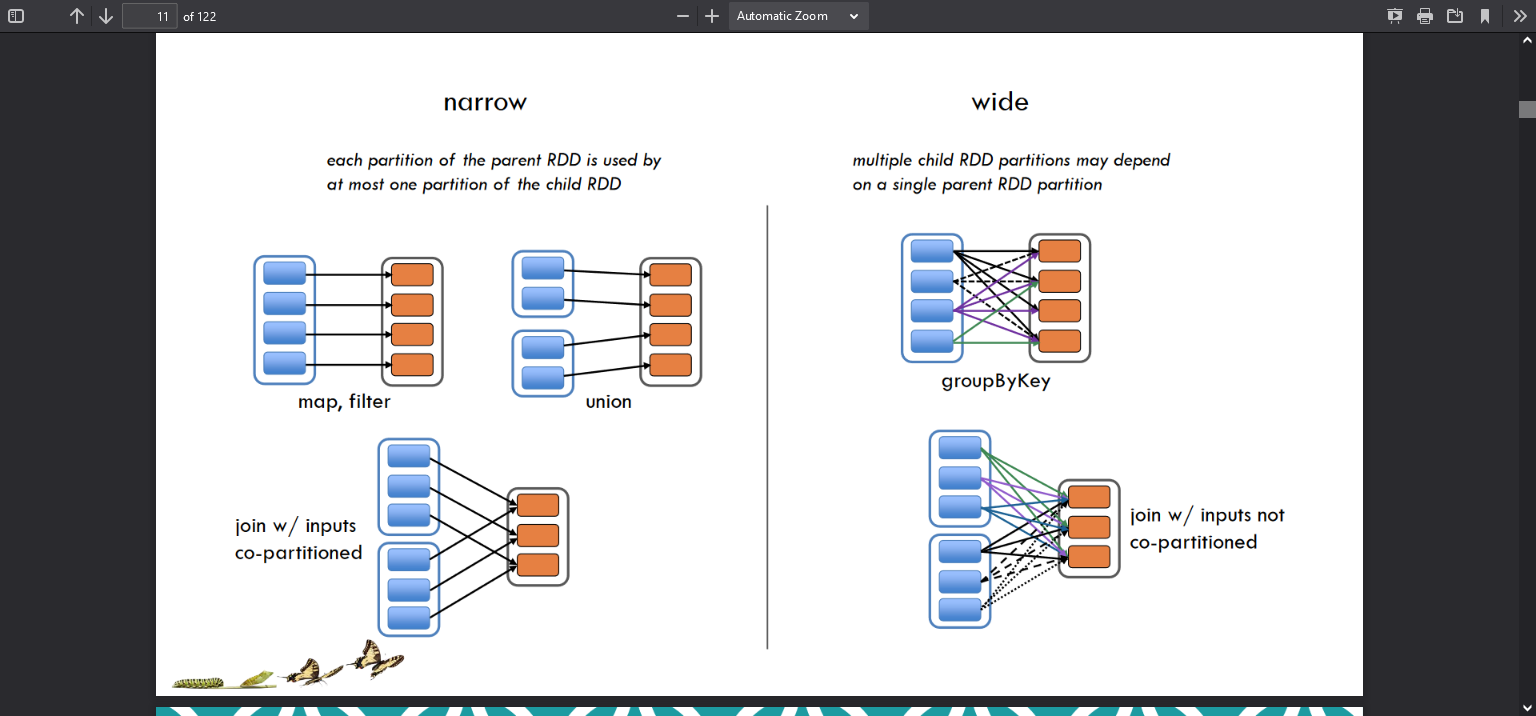
\includegraphics[scale=0.5]{images/transformActionPic.png}
    \caption{En fin caption}
  \end{figure}

\subsection{Transformering og handling}
Det er viktig å vite hvordan å bruke disse to forskjellige metode-typene i scala. Det viktigste er å huske at transformeringer vil forklare hva slags endringer man ønsker på hvordan data ser ut og presenteres, samt hva som hentes ut, mens handlinger vil faktisk utføre en linje kode og lagre en kopi av den ferdigbehandlede dataen. Transformeringer gjør altså ingenting før en handling kalt. Handlinger er da altså noe som vil gjøre noe med dataen, f.eks. gjøre aggregeringer eller flytte data fra et sted til et annet. 


Det finnes fire kategorier for transformeringer og handlinger:


Generelle, matematiske/statistiske, Set teori/relasjonelle og Datastruktur/I/O


\subsubsection{Narrow og Wide tranformering}
Det finnes til slutt to forskjellige varianter av transformeringer: Narrow og Wide. Narrow transformeringer er når partisjonen til forelder RDD-en brukes på det meste av en partisjon av barne RDD-en. Wide tranformering er når flere barne-RDD partisjoner er avhengige av én forelder-RDD partisjon, i tillegg vil en wide-tranformering innebære en "shuffling"(omstokking) av data fordi den samma dataen kan være tilgjengelig på flere partisjoner. Å unngå omstokking av data vil passe på ytelsen i programmet.


\subsection{Persist, broadcast og join}
Vi bruker .persist() for å bevare en kopi av dataen på spesifisert plass lokalt i systemet. Dette gjør at det er mye mer lettvint å gjenbruke dataen, da man kun gjør nødvendige kall mot databasen/oppretter verdien én gang.


\code{Scala}{code/createTableForStudent}


I denne kodebiten så har vi da hentet ut en seksjon av dataframen(DF) og brukt \lstinline{.persist(MEMORY_ONLY)} for å lagre til kun minne. Type persist settes basert på størrelsen til dataen. Deretter broadcaster vi denne DF-en, som betyr at vi sender en read-only kopi til hver av executorene som gjør en handling, som da vil fyre av persistence-kallet. Dette skjer slik pga. lazy loading.


Etter dette gjør vi en join-with på de resulterende radene, hvor de matches etter "FatherEdu" og "MotherEdu" verdiene. En join-with transformering er da en narrow-transform. Deretter flater vi ut resultatet til en dataframe og skriver til Cassandra.


Et annet bruksområde for broadcast i en join-setting er å bruke broadcast-join.


\lstinline {storDf.join(broadcast(litenDf), "id")}


Grunnen til at man kan ønske å gjøre dette er ved bruk av et større og et mindre datasett, hvor man da ønsker å dele ut de mindre datasettet til hver executor. Hver executor som sitter sin seksjon av det store settet får en kopi av det lille, og kan da utføre join-handlingen betydelig mye raskere. Spark vil bruke broadcast-join automatisk dersom dataframen er under 10mb stor.


\subsection{Neo4j MERGE}
Vi valgte så å integrere mot Neo4j med 2 datasett, og å koble disse sammen.


\code{Scala}{code/graphDBcode.scala}




